%!TEX root = ../thesis.tex

\chapter{Results}
\label{ch:results}

\section{Exploring the Data: Cluster Analysis}

\newthought{In order to better understand the player profiles,} I used the $k$-means
clustering algorithm to separate player-seasons into clusters based on their
tendencies. This algorithm works by adjusting cluster centers in order to minimize
inertia, also known as within-cluster sum of squares: $$ \sum_{i=1}^n \min_{c \in C}
\lVert x_i - \mu_c \rVert^2 $$ where $C$ is the set of clusters and $\mu_c$ is the
center of cluster $c$. The $k$-means algorithm was chosen over other clustering
algorithms for a few reasons; first, it is a simple and easy-to-understand algorithm
that often gives intuitive results and has few parameters to tune other than the
number of clusters. Second, using inertia as the loss function for clustering
assumes that clusters are convex and isotropic, which is a reasonable assumption for
player types; in other words, the shapes of a cluster of players in player profile
space should be roughly spherical, rather than elongated or oddly-shaped.

In order to apply $k$-means to the player profiles, I used player profile data from
every season from 2006-07 to 2015-16, ignoring the ``replacement player'' category
used for the regression analysis so that the 360 players involved in the most plays
in each season were considered. As noted in section~\ref{sec:profiles}, the profiles
were normalized within each year by subtracting a given season's average for each
feature and dividing by its standard deviation; this is necessary because $k$-means
treats each datum as a point in space, so it is necessary for each feature to be on
the same scale.

Next, because $k$-means weights each dimension equally in computing distances, steps
must be taken to ensure that the many offensive features do not dominate the
relatively few defensive and rebounding features when distances are computed in
$k$-means. To remedy this problem, the variances of the five defensive and two
rebounding features were inflated by factors of 2 and 3 respectively so that they
are not drowned out by variance from the 25 offensive features. While these
adjustments were ad-hoc, they yielded intuitive results; moreover, the fact that
defensive and rebounding features are correlated with some offensive features
ensures that some of this signal is encapsulated in the offensive features. For
example, both rebounding features were heavily correlated with the proportion of a
player's shots taken from within four feet of the basket, as was block rate;
similarly, steal rate is correlated with a player's field goal percentage on corner
three-point attempts.

In order to determine the optimal number of clusters $k$, the goodness of fit for
a given value of $k$ was determined by the average silhouette score over all data
points. The silhouette score for a data point $x_i$ assigned to cluster $c$ of $N_c$
points is given by
$$
\frac{b_i - a_i}{\max(a_i, b_i)}
$$
where $a_i$ is the average distance between $x_i$ and all other points in cluster
$c$ and $b_i$ is the smallest average distance between $x_i$ and the nearest cluster
to which $x_i$ does not belong:
$$
a_i = \frac{1}{N_c} \sum_{x_j \in c} \lVert x_i - x_j \rVert \qquad
b_i = \min_{c' \neq c} \frac{1}{N_{c'}} \sum_{x_j \in c'} \lVert x_i - x_j
\rVert
$$
Therefore, a silhouette score close to one indicates that the point is
well-clustered, whereas a score close to zero indicates that a point is near the
border between clusters. Thus, a good clustering will have a higher average
silhouette score than a worse clustering. The average silhouette scores for various
values of $k$ are shown in figure~\ref{fig:sils}.

\begin{figure}
    \centering
    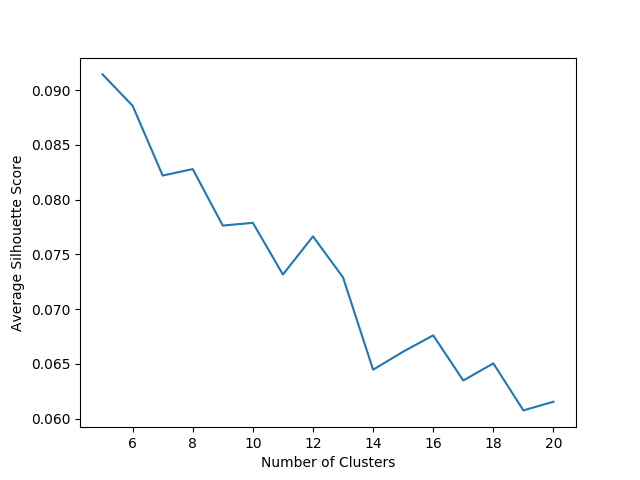
\includegraphics[width=0.75\textwidth]{figures/sil_scores}
    \caption{Average silhouette scores for various values of $k$.}
    \label{fig:sils}
\end{figure}

From this figure, $k=8$ was chosen to be the best choice for the number of clusters.
This is because there is a relatively large dropoff after $k=8$, whereas there
is actually an increase in average silhouette scores from $k=7$ to $k=8$; moreover,
while there are greater average silhouette scores for lower values of $k$, these
values are so low that the clusters would not be as interesting. For example, if
$k=5$ was chosen, then the clusters would probably have a high correlation with
the five traditional positions in basketball and thus the clustering would provide
little insight.

After re-applying the $k$-means algorithm with $k=8$, we arrive at cluster means as
shown in table~\ref{tab:clus_means}. Note that the means shown are the means of the
data that is after standardization by year but prior to inflating the variance of
the defense and rebounding features.

\begin{table}
    \centering
    \noindent\makebox[\textwidth]{%
\begin{tabular}{ccccccccc}
\toprule
    & \multicolumn{8}{c}{Cluster} \\
Feature &     1 &     2 &     3 &     4 &     5 &     6 &     7 &     8 \\
\midrule
FGA per play                   & -0.28 & -0.65 &  0.38 &  0.22 &  0.59 &  0.53 & -0.29 & -1.03\\
AST per teammate FGM           & -0.40 & -0.83 & -0.34 &  0.98 & -0.36 &  1.09 & -0.50 & -0.82 \\
FT \%                          &  0.36 & -0.67 &  0.12 &  0.20 & -0.04 &  0.62 & -0.37 & -1.42 \\
FTA per FGA                    & -0.76 &  0.55 & -0.14 & -0.03 &  0.19 & -0.23 &  0.10 &  1.47\\
PF drawn per play              & -0.89 &  0.12 &  0.03 &  0.21 &  0.66 &  0.11 & -0.08 &  0.55\\
Lost balls per play            & -0.77 & -0.03 & -0.00 &  0.36 &  0.49 &  0.40 & -0.21 & -0.08\\
Bad passes per play            & -0.39 & -0.79 & -0.29 &  0.96 & -0.32 &  0.88 & -0.33 & -0.71\\
Travels per play               & -0.41 &  0.31 &  0.13 & -0.13 &  0.52 & -0.16 &  0.24 &  0.12 \\
Offensive fouls per play       & -0.66 &  1.06 &  0.01 & -0.24 &  0.35 & -0.43 &  0.29 &  0.85\\
Percent of 2-pt FGM assisted   &  0.32 &  0.79 &  0.31 & -0.86 &  0.56 & -1.12 &  0.67 &  0.56\\
Percent of 3-pt FGM assisted   &  0.65 & -1.42 &  0.59 &  0.27 & -0.40 &  0.21 &  0.33 & -1.56\\
Percent of FGA, 2-pt $\leq$ 4 ft & -0.86 &  0.89 & -0.23 & -0.19 &  0.35 & -0.52 &  0.29 &  1.95 \\
Percent of FGA, 2-pt 5-8 ft    & -0.74 &  1.05 & -0.08 & -0.34 &  0.91 & -0.30 & -0.02 &  0.86\\
Percent of FGA, 2-pt 9-16 ft   & -0.54 &  0.53 &  0.08 & -0.15 &  0.95 &  0.14 &  0.00 & -0.56\\
Percent of FGA, 2-pt 17+ ft    &  0.08 & -0.40 &  0.20 &  0.09 &  0.07 &  0.34 &  0.29 & -1.29 \\
Percent of FGA, 3-pt $\leq$ 23 ft &  1.33 & -0.82 &  0.02 &  0.04 & -0.76 & -0.06 & -0.23 & -0.86 \\
Percent of FGA, 3-pt 24-26 ft  &  1.06 & -1.09 &  0.13 &  0.30 & -0.95 &  0.37 & -0.41 & -1.13 \\
Percent of FGA, 3-pt 27-30 ft  &  0.54 & -0.82 & -0.02 &  0.30 & -0.72 &  0.56 & -0.35 & -0.82 \\
FG\%, 2-pt $\leq$ 4 ft         & -0.20 &  0.30 &  0.20 & -0.20 &  0.47 & -0.38 &  0.14 &  0.31 \\
FG\%, 2-pt 5-8 ft              & -0.18 &  0.18 &  0.15 & -0.12 &  0.37 &  0.10 & -0.23 & -0.16\\
FG\%, 2-pt 9-16 ft             &  0.04 & -0.04 &  0.02 & -0.06 &  0.25 &  0.22 & -0.16 & -0.53\\
FG\%, 2-pt 17+ ft              &  0.13 & -0.10 &  0.14 &  0.07 &  0.21 &  0.24 & -0.02 & -1.21 \\
FG\%, 3-pt $\leq$ 23 ft        &  0.51 & -1.08 &  0.32 &  0.31 & -0.69 &  0.47 & -0.06 & -1.16 \\
FG\%, 3-pt 24-26 ft            &  0.53 & -1.32 &  0.33 &  0.33 & -0.48 &  0.50 & -0.05 & -1.25 \\
FG\%, 3-pt 27-30 ft            &  0.39 & -0.76 &  0.25 &  0.26 & -0.40 &  0.35 & -0.22 & -0.90 \\
Blocks per opponent 2-pt FGA   & -0.51 &  1.26 & -0.13 & -0.52 &  0.68 & -0.75 &  0.29 &  1.37 \\
Steals per play                & -0.24 & -0.79 & -0.46 &  1.48 & -0.51 & -0.02 &  0.31 & -0.29 \\
Personal fouls per play        & -0.34 &  1.39 & -0.28 & -0.37 & -0.03 & -0.70 &  0.61 &  1.03 \\
Opponent TO per play           & -0.07 & -0.30 & -0.46 &  0.81 & -0.46 & -0.48 &  0.94 &  0.18\\
Offensive rebounding rate      & -0.75 &  1.11 & -0.08 & -0.64 &  1.08 & -0.88 &  0.49 &  1.84 \\
Defensive rebounding rate      & -0.65 &  0.47 &  0.24 & -0.58 &  1.59 & -0.95 &  0.42 &  1.48 \\
Defensive RAPM                 &  0.03 & -0.10 & -0.43 &  0.51 & -0.01 & -0.63 &  0.60 &  0.50 \\
Offensive RAPM                 & -0.03 & -0.48 &  0.12 &  0.17 &  0.18 &  0.18 & -0.21 & -0.16 \\
\bottomrule
\end{tabular}
    }
    \caption{Player profile for the average member of each cluster, measured in
    standard deviations from the year's mean in a given feature.}
    \label{tab:clus_means}
\end{table}

Most of these clusters can be mapped intuitively to a known player type in the NBA.
For example, cluster 1 seems to represent three-point specialists like Kyle Korver
or Courtney Lee, who don't shoot often but shoot most of their shots from
three-point range, and are successful from that range; these players typically are
assisted on their shots rather than creating their own shots off the dribble.
Players in cluster 2 are capable of rebounding and protecting the rim, but are
relatively unskilled offensively other than on shots within the paint; examples
include Timofey Mozgov and Taj Gibson. The cluster mean for cluster 3 has a positive
field goal percentage from every distance on the court and takes an above average
number of shots per play; these are typically scorers who play on the wing, like
Carmelo Anthony or Tobias Harris. The fourth cluster comprises players who
facilitate their team's offense through assists, shoot well, and are very effective
on defense by forcing steals and turnovers. These are players that tend to be point
guards like Chris Paul and Rajon Rondo, but they can also come from other positions;
for example, Paul George and Kawhi Leonard belong to this cluster. Cluster 5
contains skilled offensive big men who are able to make mid-range shots and stretch
the floor, such as Kevin Love or Tim Duncan. Members of cluster 6 tend to be very
good facilitators, as they average the highest rate of assists per teammate field
goal made, while also being capable shooters and subpar defenders; examples include
Tony Parker, Isaiah Thomas, and Kyrie Irving. Cluster 7 contains bigger wings and
big men who are able to defend at a high level; the cluster includes Ersan Ilyasova
and P.J.\ Tucker.  Finally, cluster 8 mostly contains elite rebounders and rim
protectors; these are the stereotypical centers, such as Dwight Howard and DeAndre
Jordan. Understanding these clusters can be helpful in interpreting some of the
results below, where clusters allow an easy way to distill a player's profile into a
single player type; a summary of the interpretation of these clusters is given in
table~\ref{tab:clust_interp}.

\begin{table}
    \centering
    \noindent\makebox[\textwidth]{%
    \begin{tabular}{ccc}
        \toprule
        Cluster & Description & Example Player \\ \midrule
        1 & Three-Point Specialist & Kyle Korver \\
        2 & Big men with poor offensive skill & Timofey Mozgov \\
        3 & Scoring wings & Carmelo Anthony \\
        4 & Facilitator with strong defense & LeBron James \\
        5 & Floor-stretching big men & Kevin Love \\
        6 & Facilitator with poor defense & Tony Parker \\
        7 & Strong defensive wings and bigs & Ersan Ilyasova \\
        8 & Elite rebounders and rim-protectors & Dwight Howard \\
        \bottomrule
    \end{tabular}
    }
    \caption{A summary of the interpretations of the eight clusters.}
    \label{tab:clust_interp}
\end{table}


\section{Cross-Validation Results}

As explained in section~\ref{sec:mod_sel}, cross-validation was performed using data
from the 2011-12 season through the 2013-14 season; many different cross-validation
runs were done in order to tune model hyperparameters; the results are summarized in
table~\ref{tab:cv_results}.

\begin{table}
    \centering
    \noindent\makebox[\textwidth]{%
    \begin{tabular}{cc|ccc}
        \toprule
        & Optimal Hyperparameters &
        Linear Regression & Random Forests & Gradient-Boosting \\[1em]
        Optimal Hyperparameters & & N/A & \parbox[c]{3cm}{300 estimators,\\ max
        depth 3} & \parbox[c]{3cm}{300 estimators,\\ max depth 3,\\ learning
        rate 0.1} \\ \midrule
        PCA & \parbox[c]{3cm}{3 components} & 1.263605* & 1.264270 &
        1.264506 \\ \midrule
        Isomap & \parbox[c]{3cm}{5 components,\\ 5 neighbors} & 1.266315 &
        1.266019 & 1.267266 \\ \midrule
        LLE & \parbox[c]{3cm}{5 components,\\ 5 neighbors} & 1.266406 & 1.266016 &
        1.267420 \\
        \bottomrule
    \end{tabular}
    }
    \caption{A summary of the results of hyperparameter tuning and cross-validation;
    each entry in the table is the cross-validation root mean squared error for a
    given combination of dimensionality reduction and regression techniques.}
    \label{tab:cv_results}
\end{table}

Somewhat surprisingly, the regression model with the best performance in
cross-validation is the simple linear regression model. Moreover, less surprisingly,
principal components analysis beat out the nonlinear dimensionality reduction
techniques, as models trained using PCA outperformed Isomap and LLE regardless of
the regression model used. This is unsurprising, as there was no known non-flat
manifold geometry known to exist in the data. As noted in section~\ref{sec:regress},
the linear regression model does encapsulate interactions between players, to an
extent; this is because the players are sorted in order of total RAPM, so unlike the
baseline RAPM model discussed in the introduction and in section~\ref{sec:baseline},
substituting player 1 for player 2 is not as simple as adding player 1's ratings
and subtracting player 2's ratings because the substitution can result in a
shuffling of the order of the players in the regression, which in turn means that a
player's feature values may be matched with different coefficients if his position
in the sorted lineup changes as a result of the substitution. Therefore, while it is
not a nonlinear model, this linear regression model still functions differently than
the adjusted plus/minus model in that the effect of a substitution is not
necessarily the same regardless of the other players on the court as it is in the
APM model. Therefore, the model selected via cross-validation was to first use PCA
with 3 components to reduce the dimensionality of the player profiles, followed by a
simple linear regression.

\section{Comparison to Baseline Model}
\label{sec:baseline}

The motivation for this model is to incorporate play styles in order to improve upon
the regularized adjusted plus/minus model when predicting the relative performance
of two lineups. However, the (R)APM framework is used as a method for evaluating
individual players and is not used to produce predictions for two arbitrary lineups;
therefore, an extension of the model is necessary in order to adapt it to
predict the outcome of a possession. If one is to accept the RAPM model's assumption
that the point outcome of a possession can be linearly allocated to the ten players
on the court as in~\eqref{eq:apm}, then it naturally follows from the model to model
the points per possession of one lineup against another as a linear combination of
the players' RAPM ratings with a home court adjustment:
\begin{equation} \label{eqn:baseline}
    y_i = \sum_{p \in OP_i} x_{\text{off}, p} - \sum_{p \in DP_i} x_{\text{def}, p}
    + \beta_{\text{HCA}}x_{\text{HmOff},i} + \beta_{\text{const}} + \epsilon_i
\end{equation}
where $y_i$ represents points on a possession $i$, $OP_i$ and $DP_i$ are the sets of
offensive and defensive players on the court for possession $i$ respectively,
$x_{\text{off}, p}$ and $x_{\text{def}, p}$ are player $p$'s computed ORAPM and
DRAPM ratings respectively, $x_{\text{HmOff}, i}$ is an indicator for whether the
home team is on offense for possession $i$, and $\epsilon_i$ is a
normally-distributed error term with zero mean. Then, the coefficients
$\beta_{\text{HCA}}$ and $\beta_{\text{const}}$ are optimized via ordinary least
squares. Note that the ORAPM and DRAPM predictors are not given coefficients; this
is because the RAPM model inherently assumes that these ratings combine linearly
with equal weights for each player. This assumption is made by the APM model
in~\eqref{eq:apm} wherein points on a possession is modeled as equal to the sum of
the offensive players' coefficients minus the sum of the defensive players'
coefficients, using an indicator to control for home court advantage and an
intercept term to control for league-wide average efficiency. In other words, this
is essentially the same prediction that a fitted RAPM model would make, were one to
use it to predict the outcome of a possession. Therefore, this model for predicting
points per possession follows logically from the RAPM framework for player
evaluation.

Both the baseline RAPM model and the full model including the PCA-transformed player
profiles were trained on second-half possessions from the 2006-07 season through the
2013-14 season as described in chapter~\ref{ch:methods}. A comparison of these
models on a variety of metrics measuring performance on out-of-sample data from the
2014-15 and 2015-16 seasons is given in table~\ref{tab:compare}. Clearly, the model
including the transformed player profile features as predictors outperformed the
baseline model. Although the differences are small, this is largely due to the level
at which the regression is being done; that is, the upper bound on the performance
of a model that uses only play-by-play data to predict point outcomes on each
possession is quite low due to the noise and variability in possession outcomes. For
instance, both models tested here will always predict the same point outcome given
offensive and defensive lineups; however, if these two lineups play for several
possessions, they are likely to have several different point outcomes over the
course of these possessions. This error is unavoidable given the model
specifications of the RAPM model and of the player profile model. Therefore, the
model is able to improve prediction accuracy on out-of-sample data compared to the
RAPM model.

\begin{table}
    \centering
    \noindent\makebox[\textwidth]{%
    \begin{tabular}{ccc}
        \toprule
        Metric & RAPM Model & Player Profile Model \\ \midrule
        $R^2$ & 0.0001632 & 0.001962 \\
        Root Mean Squared Error & 1.29454 & 1.29440 \\
        Median Absolute Error & 1.03275 & 1.03038 \\ \bottomrule
    \end{tabular}
    }
    \caption{Comparing the out-of-sample performance of the regression on player
    profile data to the baseline RAPM model.}
    \label{tab:compare}
\end{table}

\section{Player Ratings}

Using the player profile model, a given player $p$ can be evaluated by computing the
expected point differential per possession that a team of $p$ and four replacement
players would achieve against a team of five replacement players; this assigns a
``points above replacement'' (PAR) rating based on how much a player contributes to
an otherwise replacement-level team. Expected point differential per possession is
computed by using the model to predict the points per possession when the player's
lineup is on defense and subtracting this value from the predicted points per
possession when the player's lineup is on offense; for simplicity's sake, the
offense is always assumed to be the home team, so that the home court advantage
cancels out during subtraction. Using the model trained on data from the 2006-07 NBA
season through the 2013-14 NBA season, ratings were calculated for all 297 players
who played at least 820 minutes in the 2015-16 season and were not considered
replacement-level players for the 2016 season in the player profile analysis; the
minute cutoff was chosen because it corresponds to an average of 10 minutes per game
over the 82-game season; moreover, because we are evaluating players for the
2016 season, the nine replacement players will be given the player profile for the
2016 replacement-level player. The best and worst of these ratings are shown in
table~\ref{tab:player_ratings}, which includes each player's ``points above
replacement'' over 100 possessions as well as their ORAPM, DRAPM, and total RAPM,
also prorated to 100 possessions.

\begin{table}
    \centering
    \noindent\makebox[\textwidth]{%
        \begin{tabular}{cccccc}
            \toprule
            Player & Cluster &  PAR Rating &  ORAPM &  DRAPM &  RAPM \\
            \midrule
 Russell Westbrook &       4 &   6.356 &  3.231 &  0.182 & 3.413 \\
     Stephen Curry &       4 &   5.633 &  4.124 &  1.390 & 5.515 \\
      LeBron James &       4 &   5.041 &  3.371 &  1.429 & 4.800 \\
        Chris Paul &       4 &   4.652 &  3.227 &  0.228 & 3.455 \\
      James Harden &       4 &   3.799 &  1.814 & -1.090 & 0.724 \\
      Kevin Durant &       3 &   3.645 &  3.152 &  0.924 & 4.076 \\
      Kyrie Irving &       6 &   2.841 &  2.565 & -0.848 & 1.717 \\
     Isaiah Thomas &       6 &   2.746 &  1.952 & -0.965 & 0.986 \\
    Damian Lillard &       6 &   2.225 &  1.808 & -1.463 & 0.345 \\
        Kyle Lowry &       4 &   2.071 &  1.778 &  0.471 & 2.248 \\
    Draymond Green &       7 &   2.070 &  3.045 &  2.056 & 5.101 \\
    Reggie Jackson &       6 &   1.957 &  1.310 &  0.194 & 1.504 \\
         John Wall &       4 &   1.893 &  0.848 &  0.229 & 1.077 \\
     Klay Thompson &       1 &   1.793 &  3.367 &  0.198 & 3.565 \\
     Manu Ginobili &       4 &   1.730 &  1.998 &  1.278 & 3.276 \\
            \vdots & \vdots & \vdots & \vdots & \vdots & \vdots \\
      Jerami Grant &       7 &  -5.327 & -1.389 &  0.066 & -1.323 \\
        Josh Smith &       7 &  -5.349 & -2.324 &  0.350 & -1.975 \\
   Bismack Biyombo &       8 &  -5.601 & -1.636 &  0.448 & -1.188 \\
       Noah Vonleh &       2 &  -5.622 & -1.112 & -0.765 & -1.876 \\
    Doug McDermott &       1 &  -5.740 & -0.755 & -0.437 & -1.192 \\
  Dante Cunningham &       3 &  -5.762 &  0.030 & -1.515 & -1.485 \\
     Dwight Powell &       7 &  -5.865 & -1.998 &  1.274 & -0.724 \\
      Kyle Singler &       1 &  -6.061 & -0.755 & -0.774 & -1.529 \\
      Brandon Rush &       1 &  -6.289 & -0.565 & -1.485 & -2.051 \\
     Rashad Vaughn &       1 &  -6.295 & -0.837 & -0.609 & -1.446 \\
      Nik Stauskas &       1 &  -6.356 & -1.703 & -1.825 & -3.528 \\
      Nerlens Noel &       8 &  -6.643 & -3.678 &  0.549 & -3.129 \\
        Alonzo Gee &       1 &  -7.151 & -1.671 & -0.455 & -2.126 \\
 Richard Jefferson &       1 &  -7.319 & -1.859 & -0.819 & -2.678 \\
   Wayne Ellington &       1 &  -7.449 & -2.404 &  0.002 & -2.402 \\
            \bottomrule
        \end{tabular}
    }
    \caption{Top fifteen and bottom fifteen players measured by expected point
    differential per 100 possessions playing with nine replacement-level players.}
    \label{tab:player_ratings}
\end{table}

There are a few things to note when interpreting these ratings. First, recall that
player profiles are built from data from both the prior season and the first half of
the season in question; therefore, these 2015-16 ratings are based partially on the
2015-16 season itself and partially on the prior 2014-15 season.  Moreover, the
motivation of the player profiles model is to evaluate how the play styles of the
members of a lineup interact with each other, so having a low rating in
table~\ref{tab:player_ratings} simply indicates that the player would not contribute
well to a team of replacement-level players against a team of replacement-level
players.  However, it is still possible that the same player would be an effective
contributor to different lineups or against different lineups.

That said, the results of the model are very interesting. First, the names at the
top of the list should be familiar to even the casual NBA fan; this is a good sanity
check, as Russell Westbrook, Steph Curry, and LeBron James were widely considered
the best three players in the league in 2016, and Curry won MVP for his performance.
However, he did not earn the top spot according to the model; instead, Westbrook
edged out Curry by about 0.7 points per 100 possessions. An intuitive explanation
for this is that, when playing with only replacement players, it is important to be
able to score and rebound for oneself without relying on mediocre teammates.  When
inspecting their player profiles, one finds that Russell Westbrook's top attribute
is assist rate, or the percentage of teammate field goals on which he assists while
he's on the floor, and his lowest attributes are the percent of his two-point field
goals that are assisted and the percent of his three-point field goals that are
assisted. In other words, Westbrook is elite at both helping others score and at
generating offense on his own; these are the two most important offensive skills
when playing with replacement-level players, whereas Steph Curry, while also elite
in both categories, relies slightly more on being assisted on his three-point shots.
This can likely be attributed to the Warriors' superior lineup and their style of
play, which emphasizes ball movement.

Overall, the top of the list is littered with players from the fourth and sixth
clusters. As mentioned previously, these are the clusters that emphasize
facilitating on offense; in fact, these are the only clusters that had means with
above-average assist rates. This suggests that, when playing with replacement-level
players, having an elite point guard is critical, presumably because they are able
to elevate the level of their teammates. Indeed, inspecting these players' player
profiles shows that many of them have some of the lowest rates of being assisted on
two-point field goals in the league; this typically means that they are able to
score on their own and that they deliver a large portion of their team's assists.
The only players in the top fifteen who are not in one of the two clusters are Kevin
Durant, who is perhaps the best pure scorer in the NBA, Draymond Green, whose
combination of offensive and defensive prowess is virtually unmatched, and Klay
Thompson, who is one of the best pure shooters to ever play in the NBA.

On the other hand, seven of the bottom eight players belong in the ``three-point
specialist'' category. As mentioned above, these players tend to require assists to
set up their shots. When playing with replacement-level players who tend to be bad
at facilitating, the primary strength of a three-point specialist is significantly
weakened. As a result, these players falter horribly when playing with only
replacement-level players.

\section{Lineup Ratings} \label{sec:lineup_ratings}

Just as players are evaluated by comparing them to replacement level, lineups can be
evaluated using the model by computing a lineup's expected point differential per
possession against a lineup of five replacement players. The 100 lineups with the
most possessions played in the 2015-16 season were evaluated, and the results are
given in table~\ref{tab:lineup_ratings}. Note again that 2016 replacement players
were used as the opposing team.

\begin{table}
    \centering
    \noindent\makebox[\textwidth]{%
        \begin{tabular}{cccccccc}
\toprule
       Player 1 &    Player 2 &   Player 3 &     Player 4 &       Player 5 &    Cluster Types &  Total RAPM &  Rating \\
\midrule
      H. Barnes &    S. Curry &   D. Green &  A. Iguodala &    K. Thompson &  (3, 4, 7, 1, 1) &      17.580 &  42.345 \\
       S. Curry &    F. Ezeli &   D. Green &  A. Iguodala &    K. Thompson &  (4, 8, 7, 1, 1) &      17.922 &  40.757 \\
      H. Barnes &    S. Curry &   F. Ezeli &     D. Green &    K. Thompson &  (3, 4, 8, 7, 1) &      15.597 &  39.483 \\
       A. Bogut &    S. Curry &   D. Green &  A. Iguodala &    K. Thompson &  (8, 4, 7, 1, 1) &      17.154 &  39.105 \\
      H. Barnes &    A. Bogut &   S. Curry &     D. Green &    K. Thompson &  (3, 8, 4, 7, 1) &      14.829 &  36.398 \\
      K. Irving &    L. James &    K. Love &     J. Smith &    T. Thompson &  (6, 4, 5, 1, 8) &      10.743 &  36.383 \\
       S. Adams &   K. Durant &   S. Ibaka &   D. Waiters &   R. Westbrook &  (8, 3, 3, 6, 4) &      10.966 &  36.260 \\
     B. Griffin &   D. Jordan &    L. Mbah &      C. Paul &      J. Redick &  (3, 8, 7, 4, 1) &      11.361 &  35.205 \\
 M. Dellavedova &    L. James &    K. Love &     J. Smith &    T. Thompson &  (1, 4, 5, 1, 8) &      12.355 &  34.864 \\
       A. Bogut &    S. Curry &   D. Green &      B. Rush &    K. Thompson &  (8, 4, 7, 1, 1) &      12.240 &  34.570 \\
      K. Irving &    L. James &    K. Love &    T. Mozgov &       J. Smith &  (6, 4, 5, 2, 1) &       8.069 &  34.159 \\
       S. Adams &   K. Durant &   S. Ibaka &  A. Roberson &   R. Westbrook &  (8, 3, 3, 7, 4) &      12.504 &  33.594 \\
     B. Griffin &   D. Jordan &    C. Paul &    J. Redick &  L. Stephenson &  (3, 8, 4, 1, 3) &       8.417 &  33.593 \\
    J. Crawford &  W. Johnson &  D. Jordan &      C. Paul &      J. Redick &  (6, 1, 8, 4, 1) &       8.761 &  33.587 \\
      D. Jordan &     L. Mbah &    C. Paul &    P. Pierce &      J. Redick &  (8, 7, 4, 1, 1) &       9.481 &  33.092 \\
\vdots & \vdots & \vdots & \vdots & \vdots & \vdots & \vdots & \vdots \\
 G. Antetokounmpo &       O. Mayo &  K. Middleton &    J. Parker &   M. Plumlee &  (3, 1, 4, 3, 2) &      -0.931 &  17.845 \\
       E. Bledsoe &   T. Chandler &     B. Knight &    M. Morris &    P. Tucker &  (4, 8, 6, 7, 7) &      -3.743 &  17.399 \\
     W. Ellington &    J. Johnson &      B. Lopez &     D. Sloan &     T. Young &  (1, 6, 2, 6, 5) &      -3.988 &  16.835 \\
       N. Bjelica &      G. Dieng &     Z. LaVine &    K. Martin &  S. Muhammad &  (7, 5, 6, 6, 3) &      -5.712 &  16.317 \\
         G. Dieng &     T. Prince &      R. Rubio &     K. Towns &   A. Wiggins &  (5, 1, 4, 5, 6) &      -0.746 &  15.583 \\
        A. Baynes &      S. Blake &    S. Johnson &    M. Morris &  A. Tolliver &  (2, 6, 3, 1, 1) &       0.790 &  15.542 \\
       K. Garnett &     T. Prince &      R. Rubio &     K. Towns &   A. Wiggins &  (7, 1, 4, 5, 6) &       1.791 &  15.439 \\
        K. Bryant &   J. Clarkson &    R. Hibbert &    J. Randle &  L. Williams &  (6, 6, 2, 5, 6) &     -11.552 &  14.621 \\
       A. Bradley &    J. Jerebko &     K. Olynyk &     M. Smart &    E. Turner &  (1, 7, 7, 4, 4) &       1.369 &  14.376 \\
        D. Booker &   T. Chandler &     B. Knight &       A. Len &    P. Tucker &  (6, 8, 6, 8, 7) &      -5.648 &  13.933 \\
       C. Aldrich &   J. Crawford &    W. Johnson &  P. Prigioni &    A. Rivers &  (8, 6, 1, 4, 6) &      -3.865 &  13.794 \\
    B. Bogdanovic &  W. Ellington &      B. Lopez &     D. Sloan &     T. Young &  (1, 1, 2, 6, 5) &      -6.243 &  13.633 \\
        K. Bryant &   J. Clarkson &    R. Hibbert &     L. Nance &  L. Williams &  (6, 6, 2, 7, 6) &      -9.438 &  13.532 \\
        D. Booker &   T. Chandler &        A. Len &     R. Price &    P. Tucker &  (6, 8, 8, 4, 7) &      -3.679 &  12.691 \\
        K. Bryant &   J. Clarkson &    R. Hibbert &    J. Randle &   D. Russell &  (6, 6, 2, 5, 6) &     -10.898 &  12.536 \\
\bottomrule
        \end{tabular}
    }
    \caption{Top fifteen and bottom fifteen lineups by expected point differential
    against replacement players, out of the 100 lineups that played the most
    possessions in 2015-16.}
    \label{tab:lineup_ratings}
\end{table}

These results are very reasonable and unsurprising. First, it is unsurprising that
the Warriors' so-called ``Lineup of Death'' featuring Steph Curry, Draymond Green,
Klay Thompson, Harrison Barnes, and Andre Iguodala was rated the best lineup versus
replacement players; this lineup gained notoriety during the 2015-16 season as it
became the Warriors' third most used lineup as it played 173 minutes for a
staggering +44.4 net points per 100 possessions, a couple points higher than the
player profile model's estimate against replacement-level players \cite{Ringer,
BKRef}.  After this lineup follow several other Warriors lineups, with a smattering
of Thunder, Clippers, and Cavaliers lineups rounding out the top 15. What is more
interesting about these ratings, however, is the correlation between successful
lineups and lineup composition in terms of cluster types. The majority of the highly
rated lineups contain at least one three-point specialist from cluster 1, and in
many cases two such specialists. The only lineups that do not contain a three-point
specialist are the two Thunder lineups; however, Kevin Durant is an exception in
cluster 3 in that he is an excellent three-point shooter, despite the cluster mean.
This demonstrates the importance of having players who are threats from beyond the
3-point arc.

It is also interesting to note that the total RAPM of a lineup is not completely
correlated with the lineup's points above replacement rating. For example, the
second Thunder lineup has a far lower total RAPM than the Cavaliers lineup
featuring Mozgov, but the Mozgov lineup is ranked higher than the Thunder lineup
because, according to the model, it is able to take better advantage of
complementary skill sets.

On the other side of the table are several Lakers lineups featuring a 37-year-old
Kobe Bryant; these lineups are rated very poorly and do not have any three-point
specialists on them. Also noteworthy is the number of Timberwolves lineups in the
bottom 15 lineups; in particular, the lineup of Rubio, Wiggins, Prince, Garnett, and
Towns has a positive total RAPM, almost 10 more points per 100 possessions than the
get moreworst Lakers lineup by RAPM, and yet they are projected to perform quite
poorly against replacement players, relative to the other teams.

\section{Matchups Between Starting Lineups}

Another useful application of the model is that we can test how well we would expect
each team's starting lineup to perform offensively and defensively against every
other team's starting lineup from the 2015-16 season. In order to determine a team's
starting lineup, I selected whichever lineup started the most games for a team
during the season. The expected points per possession for each possible matchup is
given in figure~\ref{fig:off_def_mat}, where the rows indicate the team on offense
and the columns indicate the team on defense; the values in the table represent the
how many points per 100 possessions the offensive lineup would be expected to score
against the defensive lineup. Note that values on the diagonal represent how well a
given team's starting lineup would be expected to fare against itself.

\begin{figure}
    \centering
    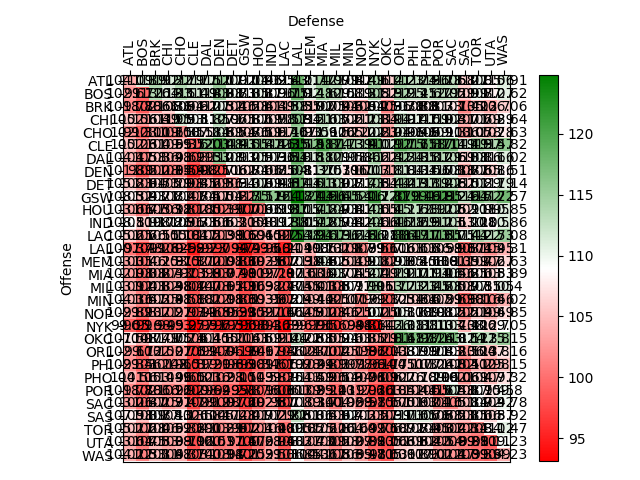
\includegraphics[width=\textwidth]{figures/off_def_matrix}
    \caption{How different teams' starting lineups would be expected to perform
    against one another on a given side of the ball.}
    \label{fig:off_def_mat}
\end{figure}

Further, for any two teams, we can compute the difference between the offensive
advantages each team was expected to have against the other based on
figure~\ref{fig:off_def_mat}. This gives an overall expected point differential per
possession for each matchup; these overall expected point differentials per
possession, prorated to 100 possessions, are given in figure~\ref{fig:pd_mat}. Note
in this figure that 104.5 points per 100 possessions is roughly average in the NBA,
so the colorbar is centered at 104.5, with green representing above average and red
representing below average.

\begin{figure}
    \centering
    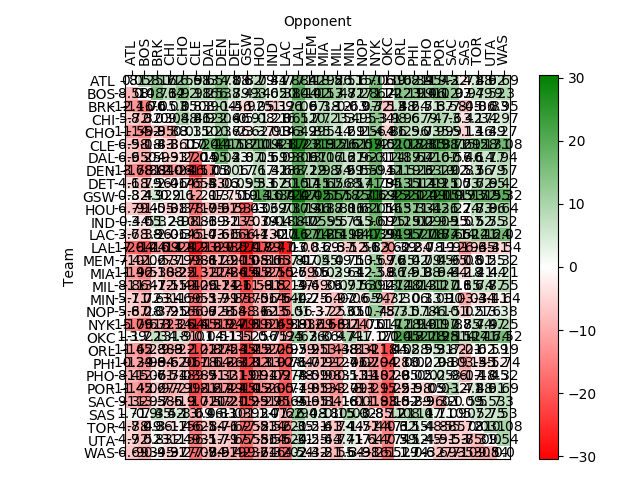
\includegraphics[width=\textwidth]{figures/point_diff_matrix}
    \caption{How different teams' starting lineups would be expected to perform
    against one another, computing the point differential between the offensive and
    defensive points.}
    \label{fig:pd_mat}
\end{figure}

These figures by and large make sense; we can see that teams like Golden State,
Oklahoma City, and Cleveland are very strong, whereas teams like Philadelphia, New
York, and the Los Angeles Lakers are weaker. It is interesting to note that because
of the way that different play styles interact, these values are not transitive; in
other words, if team A has a positive expected point differential against team B and
team B has a positive expected differential against team C, it does not necessarily
mean that team A would play well against team C. For example, Boston has a very poor
expected point differential against Oklahoma City, whereas Indiana is a better
matchup with Oklahoma City. However, the model favors Boston's starting lineup
against Indiana's. Intuitively, it makes sense that a situation like this could
arise in the NBA due to different matchups and play styles within the lineups, so it
is good that the model agrees that situations like this can arise.
